\documentclass[11pt]{article}
\input{\string~/.macros}
\usepackage[a4paper, total={7in, 9in}]{geometry}
\usepackage{bbm}
\usepackage{mathrsfs} % really cursive alphabets
\usepackage{graphicx}
    \graphicspath{{./assets}}
\usepackage{hyperref}
    \hypersetup{colorlinks=true, linktoc=all, linkcolor=blue, citecolor=red}
\usepackage[backend=bibtex,sorting=none]{biblatex}
\usepackage[margin=0cm]{caption}

% random variables
\newcommand\ry{\ensuremath{\mathsf{y}}}
\newcommand\rx{\ensuremath{\mathsf{x}}}
\newcommand\rb{\ensuremath{\mathsf{b}}} 
\newcommand\rc{\ensuremath{\mathsf{c}}}
\newcommand\rz{\ensuremath{\mathsf{z}}}
\newcommand\ru{\ensuremath{\mathsf{u}}}
\newcommand\rw{\ensuremath{\mathsf{w}}}
\newcommand\rpa{\ensuremath{\mathsf{pa}}}
\newcommand\rU{\ensuremath{\mathsf{U}}}
\newcommand\rbx{\ensuremath{\mathsf{\mathbf{x}}}}
\newcommand\rby{\ensuremath{\mathsf{\mathbf{y}}}}
\newcommand\rbu{\ensuremath{\mathsf{\mathbf{u}}}}

\newcommand\bbP{\ensuremath{\mathbbm{P}}}
\newcommand\bbQ{\ensuremath{\mathbbm{Q}}}


% boldsymbols
\renewcommand\bmu{\ensuremath{\boldsymbol{\mu}}}
\newcommand\bSigma{\ensuremath{\boldsymbol{\Sigma}}}
\newcommand\bgamma{\ensuremath{\boldsymbol{\gamma}}}
\newcommand\bomega{\ensuremath{\boldsymbol{\omega}}}
\newcommand\bnu{\ensuremath{\boldsymbol{\nu}}}


% optimization, classes of functions
\newcommand\scrF{\ensuremath{\mathscr{F}}}
\newcommand\scrS{\ensuremath{\mathscr{S}}}
\newcommand\scrP{\ensuremath{\mathscr{P}}}

% independence
\newcommand{\dperp}{\ensuremath{\perp\!\!\!\perp}}
\newcommand{\ndperp}{\ensuremath{\not\!\perp\!\!\!\perp}}

% operators
\newcommand{\prox}{\ensuremath{\mathsf{prox}}}
\addbibresource{optimal_transport}

\begin{document}

\section{Optimal Transport}

The following summarizes some chapters of computational optimal transport book \cite{peyreComputationalOptimalTransport2020}.

\subsection{Monge's and Kantorovich's formulation}

Given $a,b \in \triangle^{n-1}$, where $\triangle^{n-1}$ is unit simplex. $\alpha = \sum_{i=1}^n a_i \delta_{x_i}, \beta = \sum_{j=1}^m b_j \delta_{y_i}$ are discrete measures. The optimal transport problem tries to find a map that associate each point $x_i$ to a single point $y_j$ such that masses are preserved. This corresponds to classical Monge's formulation of optimal transport
\begin{align}
    \min_{T:\sX\to\sY: T_{\#}\alpha = \beta}\,
        &\sum_{i=1}^n c(x_i, T(x_i))
\end{align}
where $c:\sX\times\sY \to\R$ is cost defined over support of measures, and that the constraints is simply that $T$ is constrained to be a pushforward from $\alpha$ to $\beta$. The problem with Monge's formulation is that the problem is combinatorial and nonconvex, so hard to solve. Kantorovich relax the deterministic nature of transport map, allowing mass at each source point split and be dispatched to multiple target points. This information is encoded in $P\in\R^{n\times m}_+$, where $P_{ij}$ describes amount of mass flowing from $x_i$ to $y_j$. The Kantorovich formulation of optimal transport for discrete measures is then
\begin{align}
    \min_{P\in\R^{n\times m}_+: P1_m = a,\, P^T1_n = b}\,
        &\inner{C}{P}
\end{align}
where the constraints specifies the set of admissible transport map to be a coupling of marginals $\alpha,\beta$ and $C\in\R^{n\times m}$ is the cost matrix, i.e. $C_{ij} = c(x_i,y_j)$. The optimization problem is a linear program and hence can be easily solved using simplex algorithm. In addition, we can instead solve the dual problem, and because of zero duality gap, equivalently solves the primal problem,
\begin{align}
    \max_{f,g\in\R^n\times\R^m: f_i+g_j \leq C_{ij}}\,
        &\inner{f}{a} + \inner{g}{b} 
\end{align}
where $f,g$ are called dual potential.

\subsection{Entropic Regularization}

Regularizing the original optimal transport problem brings computational and statistical benefits. In particular, the optimization problem can now be solved with fast matrix scaling algorithms that scales with strength of regularization. In addition, the sample efficiency for regularized problem is also superior. The entropy of coupling between two 1 dimensional discrete measure is given by
\begin{align}
    H(P)
        = -\sum_{i,j} P_{ij}(\log(P_{ij})-1)
        = - \inner{P}{\log P} + 1^TP1
\end{align}
where taking logarithm and subtraction are elementwise operations. The entropic regularized problem
\begin{align}
    \min_{P\in\R^{n\times m}_+:P1_m=a,P^T1_n=b}\,
        &\inner{P}{C} + \epsilon H(P)
    \label{eq:opt_entropic_regularized_ot}
\end{align}
We can interpret primal objective as the information projection of the Gibbs kernel $K\in\R^{n\times m}$ where $K_{ij}=e^{\frac{C_{ij}}{\epsilon}}$ onto the admissible couplings $U(a,b)=\pc{P\in\R^{n\times m}_+\mid P1_m=a,\, P^T1_n=b}$.
\begin{align}
    \inner{P}{C} - \epsilon\inner{P}{\log P)} + \epsilon 1^T P 1
        = \epsilon \inner{P}{\log\left(P \oslash e^{-C/\epsilon} \right)} - \epsilon 1^TP1 + \epsilon 1^TK1
        = \epsilon \text{KL}(P\Vert K)
\end{align}
We can solve regularized optimal transport problem with Sinkhorn algorithm \cite{cuturiSinkhornDistancesLightspeed2013}. The basic idea is to write the 1st order optimality condition for the primal variables for the Lagrangian,
\begin{align}
    \sL(P,f,g)
        &= \inner{P}{C} - \epsilon H(P) - \inner{f}{P1_m-a}- \inner{g}{P^T1_n-b} \\
    \partial \sL(P,f,g)/\partial P_{ij}
        &= C_{ij} + \epsilon \log(P_{ij}) - f_i - g_j = 0
        \quad\Rightarrow\quad
        P_{ij} = e^{(-C_{ij}+f_i+g_j)/\epsilon}
\end{align}
Note optimal $P$ can be written as scaling of Gibbs kernel row-wise by $u=e^{f/\epsilon}$ and column-wise by $v=e^{g/\epsilon}$, i.e. $P=\diag(u)K \diag(v)$. Substitute expression for $P$ into marginal constraints, get $a = \diag(u) K \diag(v) 1_m = u\odot (Kv)$ and $b = v\odot (K^T u)$. The Sinkhorn's algorithm updates $u,v$ alternatingly
\begin{align}
    u^{(\ell+1)} 
        \leftarrow a \oslash (Kv^{(\ell)}) 
    \quad\quad
    v^{(\ell+1)}
        \leftarrow b \oslash (K^Tu^{(\ell+1)})
\end{align}
Each iteration of the algorithm uses $\sO(nm)$ computation for matrix-vector products and can be accelerated to $\sO(n\log n)$ using convolution if suppport is over gridded space. See Figure (\ref{fig:plt_sinkhorn_vary_epsilon}) to visualize effect of varying the regularization strength.

\begin{center} 
\begin{figure}[h!]
    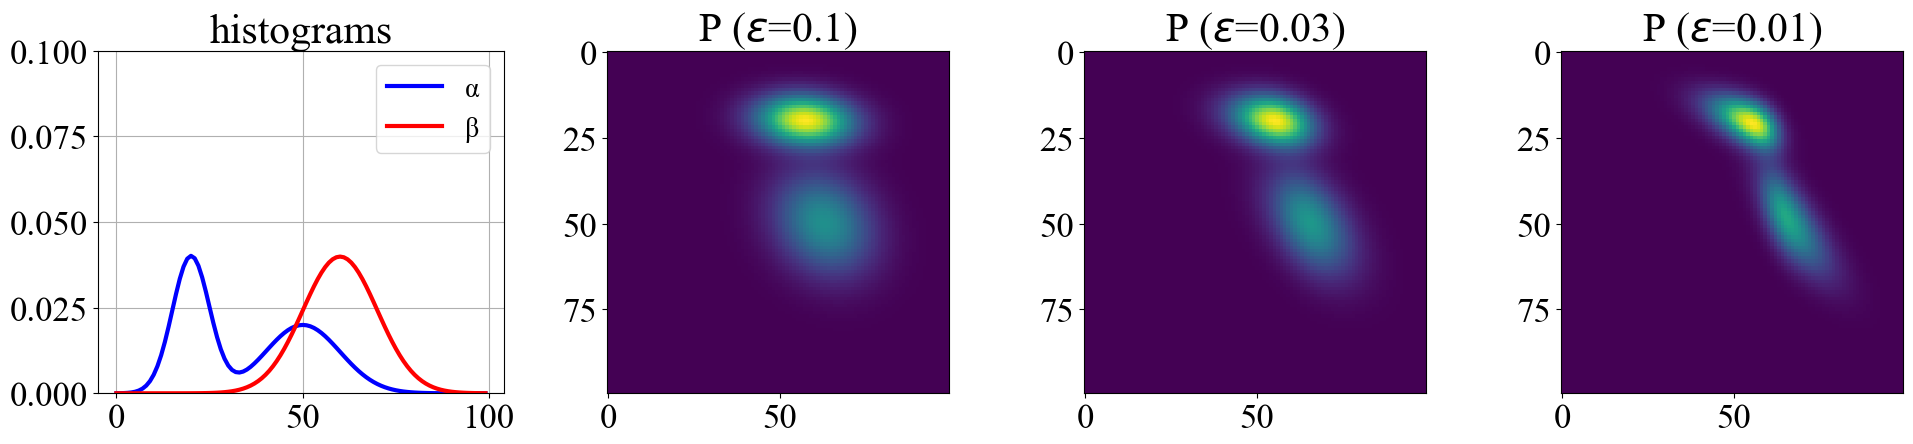
\includegraphics[width=\textwidth]{assets/plt_sinkhorn_vary_epsilon} 
    \caption{Entropic regularized optimal transport wrt 1d histograms}
    \label{fig:plt_sinkhorn_vary_epsilon}
\end{figure}
\end{center} 

Sinkhorn's iteration can be numerically unstable as $\epsilon\to 0$ due zeros in $K$, resulting in null values during division by zero. One solution is to perform computation of $u,v$ in the log-domain \cite{chizatScalingAlgorithmsUnbalanced2017, schmitzerStabilizedSparseScaling2019}. This is equivalent to block coordinate ascent on the dual of entropic regularized optimal transport problem (\ref{eq:opt_entropic_regularized_ot}),
\begin{align}
    \max_{f,g\in\R^{n\times m}} \inner{f}{a} + \inner{g}{b} - \epsilon\inner{e^{f/\epsilon}}{Ke^{g/\epsilon}}
\end{align}
Then $0 = \partial L_{\text{dual}}(f,g)/\partial f = a - e^{f/\epsilon} \odot (Ke^{g/\epsilon})$ implies $f = \epsilon \log(a) - \epsilon \log(Ke^{g/\epsilon})$ and similarly for $g$. So,
\begin{align}
    f^{(\ell+1)}
        \leftarrow \epsilon \log(a) - \epsilon\log(Ke^{g^{(\ell)}/\epsilon})
    \quad\quad
    g^{(\ell+1)}
        \leftarrow \epsilon \log(b) - \epsilon\log(Ke^{f^{(\ell+1)}/\epsilon})
    \label{eq:sinkhorn_dual_ascent}
\end{align}
This is equivalent to Sinkhorn's iteration in log domain. Additionally, we can define a numerically stable softmin operator based on log-sum-exp, $\text{softmin}_{\epsilon}(z) = - \epsilon \log \sum_{i} e^{-z_i/\epsilon} = -\epsilon \text{LSE}(-z/\epsilon)$. Note $f_i = \epsilon \log a_i - \epsilon \log \sum_j e^{-(C_{ij}-g_j)/\epsilon} =\text{softmin}_{\epsilon}(C_{ij}-f_i-g_j) + f_i +  \epsilon \log a_i$. Therefore, (\ref{eq:sinkhorn_dual_ascent}) can be equivalently written as,
\begin{align}
    f^{(\ell+1)}
        &\leftarrow \text{softmin}_{\epsilon} (S(f^{(\ell)}, g^{(\ell)})) + f^{(\ell)} + \epsilon \log(a) \\ 
    g^{(\ell+1)}
        &\leftarrow \text{softmin}_{\epsilon} (S(f^{(\ell+1)}, g^{(\ell)})) + g^{(\ell)} + \epsilon \log(b)
    \label{eq:sinkhorn_dual_ascent2}
\end{align}
where $S(f,g)_{ij} = C_{ij}-f_i-g_j$. Figure (\ref{fig:plt_sinkhorn_vary_epsilon}) is computed using log domain stabilization, where choice of $\epsilon=.001$ would yield null values without log domain stabilization.
 
\begin{center} 
\begin{figure}[h!]
    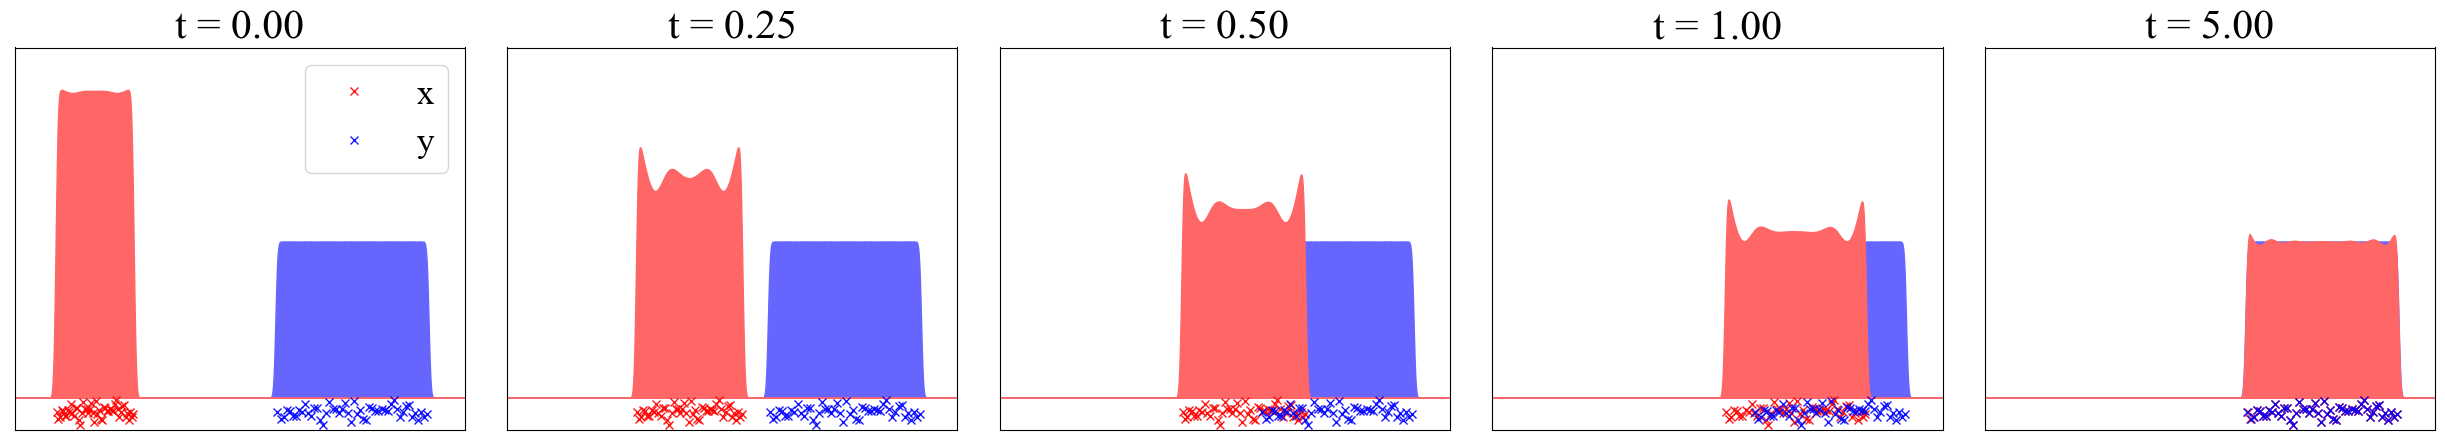
\includegraphics[width=\textwidth]{assets/plt_gradientflow1d} 
    \caption{Gradient flow of Sinkhorn divergence wrt support $x$}
    \label{fig:plt_gradientflow1d}
\end{figure}
\end{center} 
 

\subsection{Unbalanced Transport}

We can extend optimal transport to general measures by enforcing soft constraints on the coupling \cite{chizatScalingAlgorithmsUnbalanced2017},
\begin{align}
    \min_{P\in\R^{n\times m}_+}\, 
        \inner{P}{C} + \epsilon H(P) + \rho \text{KL}(P1_m \Vert a) + \rho \text{KL}(P^T 1_m \Vert b)
\end{align}
Similar to balanced case, we can show that optimal coupling is again a scaling of $K$, i.e. $P = \diag(u) K \diag(v)$ where $u = (a \oslash (Kv))^{\lambda}$ and $v = (b \oslash (K^T u))^{\lambda}$ where $\lambda = \frac{\rho}{\rho + \epsilon}$ \cite{frognerLearningWassersteinLoss2015}. We can derive a similar Sinkhorn iteration in the log domain for unbalanced case.








\newpage
\printbibliography 




\end{document}
